\section{Markstein and More}


\begin{figure}[t]
    \centering
    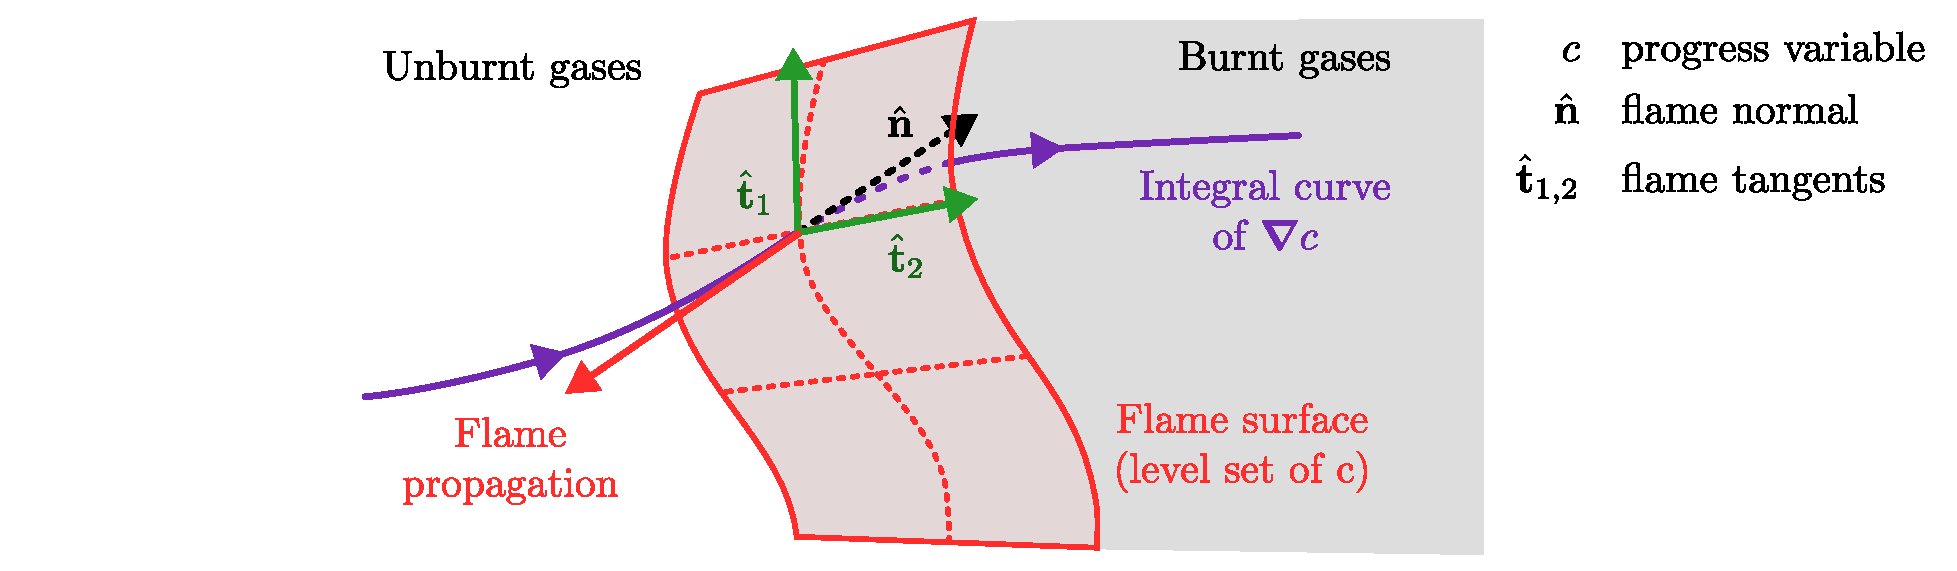
\includegraphics[scale=0.43]{assets/flamelet.pdf}
    \label{fig:flamelet}
    \caption{Diagram of the 3D flame surface model used below.}
\end{figure}

Defining the inverse thermal Peclet number: $\d = l_\rm{th} / L$ as the asymptotic parameter used by \cite{pelce1982InfluenceHydrodynamicsDiffusion,matalon1982FlamesGasdynamicDiscontinuities} to describe flame thickness alongside the Zeldovich number $\Ze$ which loosely prescribes reaction zone thickness relative to the flame thickness, the work of \cite{pelce1982InfluenceHydrodynamicsDiffusion,matalon1982FlamesGasdynamicDiscontinuities} primarily finds that the incompressible Navier-Stokes (NS) equations are suitable approximations of gas flow on either side of a premixed deflagration which is deficient in one reactant:
\begin{subequations}
\begin{boxaliat}{2}
\label{eqn:hydro-incomp} \vec{\nabla}\cdot\vec{u} &= 0                         &&+ \cl{O}\left( \d^2 \right), \\
\label{eqn:hydro-u} \r \mdv{\vec{u}}{t} &= - \vec{\nabla}p + \d\Pr \lap\vec{u} &&+ \cl{O}\left( \d^2 \right).
\end{boxaliat}
\end{subequations}
So these equations are valid on either side of the flame, which we describe mathematically by the level set of a function $F = 0$. The asymptotic papers make the additional assumption that this level set looks like the graph of a function in $y$, $f(y, t)$, such that e.g. in two-dimensions $F \equiv x - f(y, t)$. For numerical purposes, it is usually easiest to define this level set via the progress variable:
\begin{equation}
c \equiv \frac{Y_\a - Y_{\a, 1}}{\bbra{Y_\a}_V}
\end{equation}
for one of the species $\a$, so $F \equiv c - c^*$. The graph assumption is not the case for flames typically, so we instead rely on the level set formulation.

The \emph{product-pointing} normal (i.e. the normal which points towards the hot, light reaction products) is easily defined by:
\begin{equation}
\uvec{n} \equiv \frac{\vec{\nabla}c}{\norm{\vec{\nabla}c}} \bigg|_{F^-}.
\end{equation}
which is the unit normal vector pointing forward along the integral curve of $\vec{\nabla} c$ which goes through the relevant point at the flame surface. The reactant-pointing normal may also be used, which just results in a change in sign. We use the product-pointing normal so we start off without negatives. The absolute speed of the flame at a point on the flame is the component of the flame motion $\ndt{\vec{f}}$ which moves away from the products:
\begin{subequations}
\begin{equation}
S_a \equiv - \ndt{\vec{f}} \cdot \uvec{n},
\end{equation}
and the displacement speed also considers the effect of the fluid moving at the products, opposing flame motion:
\begin{equation}
S_d \equiv (\vec{u} - \ndt{\vec{f}}) \cdot \uvec{n} \,\big|_{F^-} = S_a + \vec{u} \cdot \uvec{n} \,\big|_{F^-}.
\end{equation}
Hence, considering the advection equation for the flame: $\partial c / \partial t + \ndt{\vec{f}}\cdot \vec{\nabla}c = 0$ we find the following simple expressions for absolute and displacement speed:
\begin{align}
S_a &= \frac{1}{\norm{\vec{\nabla}c}} \pdv{c}{t} \,\bigg|_{F^-} \\
S_d &= \frac{1}{\norm{\vec{\nabla}c}} \mdv{c}{t} \,\bigg|_{F^-}
\end{align}
In this context, the species conservation equation may be used:
\begin{align}
\r \mdv{c}{t} &= \frac{1}{\bbra{Y_\a}_V} \cdot \r \mdv{Y_\a}{t} = \frac{1}{\bbra{Y_\a}_V} \left( \ndt{\vr}_\a - \vec{\nabla} \cdot (\r \vec{V}_{\!\a} Y_\a) \right), \\
\implies \quad \Aboxed{ S_d &= \frac{1}{\r \norm{\vec{\nabla}c} \bbra{Y_\a}_V} \left[ \ndt{\vr}_\a - \vec{\nabla} \cdot (\r \vec{V}_{\!\a} Y_\a) \right] \bigg|_{F^-} . }
\end{align}
\end{subequations}

It was primarily the work of Markstein in his seminal papers \cite{markstein1951ExperimentalTheoreticalStudies,markstein1953InstabilityPhenomenaCombustion,markstein1964NonsteadyFlamePropagation} which brought forth the idea that changes in flame speed away from its \emph{unstretched} speed, the laminar flame speed, is proportional to the amount of stretching that the flame experiences. Although Markstein first suggested a simple relationship between flame speed and curvature, it is now accepted that, at least in the hydrodynamically unstable regime, a dependence with the full \emph{flame stretch} is required. The dimensional and non-dimensional forms of these relations for consumption and displacement speed therefore follow: 
\begin{subequations}
\begin{alignat}{4}
S_{c/d}   &= S_L &&+ l_\rm{th} \Mk_{c/d}&&( -\bb{K}   &&) \\
S_{c/d}^* &= 1   &&+        \d \Mk_{c/d}&&( -\bb{K}^* &&)
\end{alignat}
\end{subequations}
with $\bb{K}$ being the flame stretch as elaborated in \cite{matalon1982FlamesGasdynamicDiscontinuities,candel1990FlameStretchBalance,clavin1985DynamicBehaviorPremixed}. This flame stretch obeys the formula:
\begin{subequations}
\begin{align}
(-\bb{K}) &= S_a (\vec{\nabla}\cdot\uvec{n}) + \uvec{n} \cdot \vec{\nabla} \cross (\vec{u}\cross \vec{n}) \Big|_{F^-} \\
&= S_d (\vec{\nabla}\cdot\uvec{n}) + \left[ (\uvec{n}\otimes\uvec{n}) : \vec{\nabla}\vec{u} - \vec{\nabla} \cdot \vec{u} \right] \Big|_{F^-} \\
&= S_d (\vec{\nabla}\cdot\uvec{n}) + \left(\uvec{t}_1\otimes\uvec{t}_1 + \uvec{t}_2\otimes\uvec{t}_2\right) : \bb{E} \,\Big|_{F^-} \\
&= S_d \kappa + E
\end{align}
\end{subequations}
depending on the flame's displacement speed, curvature $\k$ and strain $E$:
\begin{subequations}
\begin{align}
\kappa &\equiv \vec{\nabla}\cdot\uvec{n}, \\
E &\equiv \left(\uvec{t}_1\otimes\uvec{t}_1 + \uvec{t}_2\otimes\uvec{t}_2\right) : \bb{E} \,\Big|_{F^-} = \left[ (\uvec{n}\otimes\uvec{n}) : \vec{\nabla}\vec{u} - \vec{\nabla} \cdot \vec{u}\right] \, \Big|_{F^-}, \\
\bb{E} &= \frac{1}{2}\left(\vec{\nabla}\vec{u} + (\vec{\nabla}\vec{u})^T\right)
\end{align}
where $\bb{E}$ is the strain rate tensor and the vectors $\uvec{n}$, $\uvec{t}_1$ and $\uvec{t}_2$ form a moving frame on the flame surface (assuming a three-dimensional system):
\begin{equation}
\uvec{t}_{1, 2} \cdot \uvec{n} = 0
\quad \text{and} \quad
\uvec{t}_{1} \cdot \uvec{t}_2 = 0.
\end{equation}
\end{subequations}
Finally, the values $\Mk_{c/d}$ are the \emph{Markstein numbers} for the consumption and displacement speed of the flame. Classic formulae used for these values are known as the \emph{Clavin-Williams formulae} \cite{clavin1982EffectsMolecularDiffusion}:
\begin{subequations}
\begin{alignat}{2}
\Mk_d &= \Mk_1 + && \frac{1}{2}\Ze (\Le - 1) \Mk_2, \\
\Mk_c &=         && \frac{1}{2}\Ze (\Le - 1) \Mk_2,
\end{alignat}
\end{subequations}
placeholder
\begin{subequations}
\begin{alignat}{2}
\Mk_1 &\equiv \frac{1 + q}{q} \ln (1 + q)             && > 0, \\
\Mk_2 &\equiv \int_{-\infty}^0 \ln (1 + q e^x) \dd{x} && > 0.
\end{alignat}
\end{subequations}


% jump conditions (use matalon independent flame equations)
% enhancement factors
% Local flame speeds etc.
% integral curves, contours and averaged vs summed local speeds




\section{Own Work}

\begin{figure}[t]
    \centering
    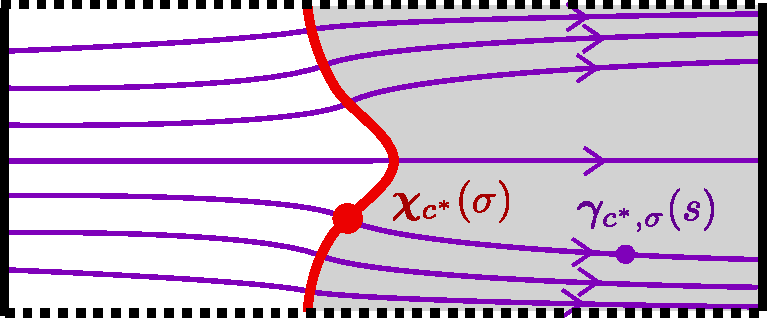
\includegraphics[scale=0.43]{assets/2d-flame-int-curves.pdf}
    \label{fig:int-curves}
    \caption{caption}
\end{figure}

These are sets depending on time, $t$, which we ignore below for brevity
\begin{subequations}
\begin{alignat}{2}
\chi_{c^*}       &\equiv \Big\{ \vec{\chi}_{c^*}(\sigma)  \, &&| \  c\big(\vec{\chi}_{c^*}(\sigma)\big) = c^* \Big\} \\
\g_{c^*, \a} &\equiv \Big\{ \vec{\g}_{c^*, \s}(s) \, &&| \  \vec{\g}_{c^*, \s}' =  \vec{\nabla}c / \norm{\vec{\nabla}c} \big|_{\vec{\g}_{c^*, \s}} \ \text{and} \  \vec{\g}_{c^*, \s}(0) = \vec{\chi}_{c^*}(\sigma) \Big\}
\end{alignat}
\end{subequations}
we find that the set integral curves does not change with time or the contour progress variable $c^*$ and covers domain:
\begin{subequations}
\begin{align}
A &= \big\{ \vec{\g}_{c_1, \s_1}(s_1) \, | \ s_1, \ \s_1 \ \text{and} \ \vec{\g}_{c_1, \s_1} \in \g_{c_1, \s_1} \big\} \\
&= \big\{ \vec{\g}_{c_2, \s_2}(s_2) \, | \ s_2, \ \s_2 \ \text{and} \  \vec{\g}_{c_2, \s_2} \in \g_{c_2, \s_2} \big\}
\end{align}
\end{subequations}
where $c_1 \neq c_2$. This ensures that integral quantities over the whole domain $A$ are exactly calculated by the continuous summation of integrals of the same quantity over each integral curve. For consumption speed $S_c$, this means that:
\begin{equation}
S_{c, \rm{loc}}(\s) = \frac{1}{\r_1 \bbra{T}_A} \int_{s_1}^{s_2} \frac{\ndt{\cl{T}}(\s, s)}{c_p(\s, s)} \dd{s},
\quad \text{and} \quad
\overline{S_{c, \rm{loc}}} = \frac{1}{L[\chi]} \int_{\s_1}^{\s_2} S_{c, \rm{loc}}(\s) \dd{\s}
\end{equation}
so
\begin{subequations}
\begin{align}
S_c &= \frac{1}{w \r_1 \bbra{T}_A} \int_A \frac{\ndt{\cl{T}}}{c_p} \dd{A} = \frac{1}{w \r_1 \bbra{T}_A} \int_{\s_1}^{\s_2} \int_{s_1}^{s_2} \frac{\ndt{\cl{T}}(\s, s)}{c_p(\s, s)} \dd{s} \dd{\s} \\
&= \frac{1}{w} \int_{\s_1}^{\s_2} S_{c, \rm{loc}}(\s) \dd{\s} = \frac{L[\chi]}{w} \cdot \overline{S_{c, \rm{loc}}}
\end{align}
\end{subequations}

% This means that integral quantities over the whole domain (S_c) can be exactly calculated through integrals over the curve of the same integral values (S_c,loc) over individual integral curves
% For S_c this turns out to be: integral over area = integral over x then y = integral over integral curve then contour

% Our contour finding algorithm is the marching squares algorithm which, as the name suggests, requires a cartisian grid of input data. We interpolate our unstructured mesh-free nodes onto a cartesian grid using cubic splines. Analyse only the DNS nodes which are in a rectangle around the flame so as to be non-negligible to same computational time. The contours may then be found for any progress variable c^*. The chemical progress variable c_Y was chosen here for the same reasons as Day et al and Howarth 2022 to better represent flame locations and reduce closed loop contours (C_Y = C_T FOR IDEALISED FLAMES, THEY HAVE NON-IDEALISED FLAMES). Note that the choice of the flame location is entirely arbitrary as a function of a continuous progress variable (in the asymptotic regime we essentially have discontinuous progress variable c = 0, the reactants, and c = 1, the products) so we are forced to make some sensible choice. we call this choice the flame progress variable c_flame, and take it to be a value of progress variable which best represents the location of highest heat release. Any other 'metric' could be used justifiably, and we hope at this stage that the value of the Markstein number is independent of this choice
% On this flame contour, normals may be calculated by travelling short distances along integral curves and used to calculate rate of strain and curvature. To calculate curvature we use a two point finite difference stencil:

% Rate of strain is calculated by the formula ( -- ) where spatial derivatives are easily calculated on the interpolated data via finite differences on the mesh points. Theoretically, rate of strain is evaluated just ahead of the flame, at f^-. In the context of simulation data this is again ambiguous as above, so we must choose its location. Normals are already treated to represent the shape of the flame, but for the upstream hydrodynamics, we must use some other metric. Hence, we choose to use a smaller progress variable, more representative of the reactant mixture location at the beginning of reaction, c_up. Rate of strain and all other evaluations of u will take place at the intersection of the c = c_up contour and the relevant integral curve. Note that we could instead evaluate values using a threshold density, but this is equivalent to using a temperature-based progress variable value.

% Flame thicknesses may be evaluated for each integral curve too. In Howarth and Aspden 2022 they have strong turbulence effects so the flame thickness vary significantly between integral curves. For these idealised laminar flames, however, we find that the flame thicknesses do not change significantly (1% or something?) so diffusive thicknesses are used unlike Howarth

% Displacement speed may be evaluated as in the previous section (equation 20f), but the evaluation of diffusive fluxes from the interpolated data generates spurious noise. Instead, we evaluate S_d from S_d = S_a + u . n. S_a may be simply estimated at steady states by assuming f dot is travelling horizontally, so then fdot = (u_in - S_c)e_x hat and ... 


% The mixing of u on upstream and n on flame contours may seem dubious, but actually when we do this our regression improves, justifying it quantitatively


